% Options for packages loaded elsewhere
\PassOptionsToPackage{unicode}{hyperref}
\PassOptionsToPackage{hyphens}{url}
%
\documentclass[
]{article}
\usepackage{amsmath,amssymb}
\usepackage{lmodern}
\usepackage{iftex}
\ifPDFTeX
  \usepackage[T1]{fontenc}
  \usepackage[utf8]{inputenc}
  \usepackage{textcomp} % provide euro and other symbols
\else % if luatex or xetex
  \usepackage{unicode-math}
  \defaultfontfeatures{Scale=MatchLowercase}
  \defaultfontfeatures[\rmfamily]{Ligatures=TeX,Scale=1}
\fi
% Use upquote if available, for straight quotes in verbatim environments
\IfFileExists{upquote.sty}{\usepackage{upquote}}{}
\IfFileExists{microtype.sty}{% use microtype if available
  \usepackage[]{microtype}
  \UseMicrotypeSet[protrusion]{basicmath} % disable protrusion for tt fonts
}{}
\makeatletter
\@ifundefined{KOMAClassName}{% if non-KOMA class
  \IfFileExists{parskip.sty}{%
    \usepackage{parskip}
  }{% else
    \setlength{\parindent}{0pt}
    \setlength{\parskip}{6pt plus 2pt minus 1pt}}
}{% if KOMA class
  \KOMAoptions{parskip=half}}
\makeatother
\usepackage{xcolor}
\usepackage[margin=1in]{geometry}
\usepackage{longtable,booktabs,array}
\usepackage{calc} % for calculating minipage widths
% Correct order of tables after \paragraph or \subparagraph
\usepackage{etoolbox}
\makeatletter
\patchcmd\longtable{\par}{\if@noskipsec\mbox{}\fi\par}{}{}
\makeatother
% Allow footnotes in longtable head/foot
\IfFileExists{footnotehyper.sty}{\usepackage{footnotehyper}}{\usepackage{footnote}}
\makesavenoteenv{longtable}
\usepackage{graphicx}
\makeatletter
\def\maxwidth{\ifdim\Gin@nat@width>\linewidth\linewidth\else\Gin@nat@width\fi}
\def\maxheight{\ifdim\Gin@nat@height>\textheight\textheight\else\Gin@nat@height\fi}
\makeatother
% Scale images if necessary, so that they will not overflow the page
% margins by default, and it is still possible to overwrite the defaults
% using explicit options in \includegraphics[width, height, ...]{}
\setkeys{Gin}{width=\maxwidth,height=\maxheight,keepaspectratio}
% Set default figure placement to htbp
\makeatletter
\def\fps@figure{htbp}
\makeatother
\setlength{\emergencystretch}{3em} % prevent overfull lines
\providecommand{\tightlist}{%
  \setlength{\itemsep}{0pt}\setlength{\parskip}{0pt}}
\setcounter{secnumdepth}{5}
% Place figures and tables exactly where they were called
\usepackage{float}
\floatplacement{figure}{H}
\floatplacement{table}{H}

% Recommended by the modelsummary package
\usepackage{booktabs}
\usepackage{siunitx}
\newcolumntype{d}{S[input-symbols = ()]}

% Add affiliations (title.tex needs to be called under template-partials)
\usepackage[noblocks]{authblk}
\renewcommand*{\Authsep}{, }
\renewcommand*{\Authand}{, }
\renewcommand*{\Authands}{, }
\renewcommand\Affilfont{\small}

% Add line numbers
\usepackage{lineno}
\linenumbers
\usepackage{float}
\usepackage{booktabs}
\usepackage{siunitx}

  \newcolumntype{d}{S[
    input-open-uncertainty=,
    input-close-uncertainty=,
    parse-numbers = false,
    table-align-text-pre=false,
    table-align-text-post=false
  ]}
  
\ifLuaTeX
  \usepackage{selnolig}  % disable illegal ligatures
\fi
\usepackage[]{natbib}
\bibliographystyle{plainnat}
\IfFileExists{bookmark.sty}{\usepackage{bookmark}}{\usepackage{hyperref}}
\IfFileExists{xurl.sty}{\usepackage{xurl}}{} % add URL line breaks if available
\urlstyle{same} % disable monospaced font for URLs
\hypersetup{
  pdftitle={Paper Title},
  pdfauthor={John Doe; Jeanne Doe},
  hidelinks,
  pdfcreator={LaTeX via pandoc}}

\title{Paper Title}
\author{John Doe\footnote{Department of Ghost, Random University, \href{mailto:johndoe99@ru.edu}{\nolinkurl{johndoe99@ru.edu}}} \and Jeanne Doe\footnote{Department of Magic, Highest-Ranked University, \href{mailto:jeannedoe99@hru.ac.uk}{\nolinkurl{jeannedoe99@hru.ac.uk}}}}
\date{2023-10-24}

\begin{document}
\maketitle
\begin{abstract}
This research is so awesome that you cannot reject this paper.
\end{abstract}

\newpage

\hypertarget{introduction}{%
\section{Introduction}\label{introduction}}

The issue this article addresses is \textbf{super} \emph{important}!

\begin{itemize}
\item
  \textbf{author names and year}: \citet{schlenker2009nonlinear} examined \ldots.
\item
  \textbf{author names and year in parentheses}: \citep{schlenker2009nonlinear}
\item
  \textbf{multiple citations in parentheses}: \citep{schlenker2009nonlinear, mas1995microeconomic}
\item
  \textbf{only year in parentheses}: \citeyearpar{schlenker2009nonlinear}
\end{itemize}

\hypertarget{materials-and-methods}{%
\section{Materials and Methods}\label{materials-and-methods}}

\hypertarget{data}{%
\subsection{Data}\label{data}}

The number of observations are 598 and 1376 for Zones 2 and 3, respectively.

Table \ref{tab:summary-statistics} presents summary statistics by zone.

\hypertarget{statistical-model}{%
\subsection{Statistical Model}\label{statistical-model}}

See equation \eqref{eq:eqn1} and \eqref{eq:eqn2} for the statistical models we use.

\begin{equation}
y = \beta_0 + \beta_1 x + \varepsilon
\label{eq:eqn1}
\end{equation}

\begin{align}
Y_z & = f_z(S) + g_z(N) + h_z(X,Y) + \varepsilon_z \\
& = \sum_{i=1}^k \phi_k(S) + g_z(N) + h_z(X,Y) + \varepsilon_z \label{eq:eqn2}
\end{align}

Our target coefficient is \(\beta_1\) (in-line math).

Here is the Latex way.

\begin{align}
Y_z & = f_z(S) + g_z(N) + h_z(X,Y) + \varepsilon_z \notag \\
& = \sum_{i=1}^k \phi_k(S) + g_z(N) + h_z(X,Y) + \varepsilon_z \label{eq-tex}
\end{align}

Equation (\ref{eq-tex}).

\hypertarget{results-and-discussions}{%
\section{Results and Discussions}\label{results-and-discussions}}

Table \ref{tab:reg-table} presents the regression results.

Figure \ref{fig:fig-1} presents the distribution of yields by zone.

\hypertarget{conclusions}{%
\section{Conclusions}\label{conclusions}}

bluh bluh\footnote{This is a footnote}, another bluh bluh\footnote{This is the second footnote}

\newpage

\hypertarget{figures}{%
\section*{Figures}\label{figures}}
\addcontentsline{toc}{section}{Figures}

I like Figure \ref{fig:fig-1} (flushed left) a lot.

\begin{figure}

\includegraphics[width=288px]{sample_to_pdf_files/figure-latex/fig-1-1} \hfill{}

\caption{The Distribution of Yield by Zone}\label{fig:fig-1}
\end{figure}

Figure \ref{fig:imported-plot} was imported.

\begin{figure}

{\centering 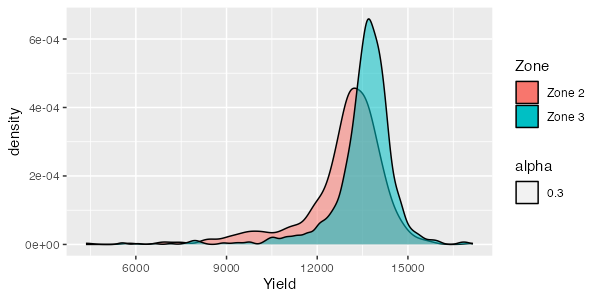
\includegraphics[width=0.2in]{g_plot_external} 

}

\caption{Imported Plot}\label{fig:imported-plot}
\end{figure}

\newpage

\hypertarget{tables}{%
\section*{Tables}\label{tables}}
\addcontentsline{toc}{section}{Tables}

\begin{table}

\caption{\label{tab:summary-statistics}Summary Statistics by Zone}
\centering
\begin{tabular}[t]{llrrrrr}
\toprule
Zone &   & get\_N & Mean & SD & Min & Max\\
\midrule
Zone 2 & Yield (kg/ha) & 598 & \num{12876.63} & \num{1445.67} & \num{4349.84} & \num{17150.77}\\
 & Nitrogen Rate (kg/ha) & 598 & \num{117.82} & \num{14.73} & \num{88.94} & \num{145.57}\\
 & Seed Rate (1000/ha) & 598 & \num{84.01} & \num{6.86} & \num{69.17} & \num{98.61}\\
Zone 3 & Yield (kg/ha) & 1376 & \num{13530.20} & \num{1093.98} & \num{5539.50} & \num{16966.78}\\
 & Nitrogen Rate (kg/ha) & 1376 & \num{118.20} & \num{14.61} & \num{88.84} & \num{143.75}\\
 & Seed Rate (1000/ha) & 1376 & \num{87.20} & \num{7.03} & \num{69.58} & \num{98.82}\\
\bottomrule
\end{tabular}
\end{table}

\begin{table}

\caption{\label{tab:reg-table}Regression results table by the modelsummary function}
\centering
\begin{tabular}[t]{lccc}
\toprule
  & (1) & (2) & (3)\\
\midrule
(Intercept) & \num{36.908} & \num{38.752} & \num{38.752}\\
 & (\num{2.191}) & (\num{1.787}) & (\num{1.857})\\
hp & \num{-0.019} & \num{-0.018} & \num{-0.018}\\
 & (\num{0.015}) & (\num{0.012}) & (\num{0.009})\\
cyl & \num{-2.265} & \num{-0.942} & \num{-0.942}\\
 & (\num{0.576}) & (\num{0.551}) & (\num{0.799})\\
wt &  & \num{-3.167} & \num{-3.167}\\
 &  & (\num{0.741}) & (\num{1.691})\\
\midrule
Num.Obs. & \num{32} & \num{32} & \num{32}\\
R2 & \num{0.741} & \num{0.843} & \num{0.843}\\
RMSE & \num{3.02} & \num{2.35} & \num{2.35}\\
Std.Errors & IID & IID & by: vs\\
\bottomrule
\end{tabular}
\end{table}

Table \ref{tab:reg-table} shows the regression results.

\newpage

\hypertarget{appendix-appendix}{%
\appendix}


\hypertarget{additional-analysis}{%
\section{Additional Analysis}\label{additional-analysis}}

\setcounter{figure}{0}
\renewcommand{\thefigure}{A.\arabic{figure}}

\begin{figure}

{\centering \includegraphics[width=468px]{sample_to_pdf_files/figure-latex/fig-a-1} 

}

\caption{The Distribution of Yield by Zone}\label{fig:fig-a}
\end{figure}

Figure \ref{fig:fig-a}.

  \bibliography{bibliography.bib}

\end{document}
